\documentclass{slides}
\usepackage[utf8]{inputenc}
\usepackage{fullpage}
\usepackage[pdftex]{graphicx}
\usepackage{epstopdf} 
\usepackage{color}
\usepackage{hyperref}
\usepackage[final]{pdfpages}
\usepackage[english]{babel}

\usepackage{verbatimbox}
\usepackage{fancyvrb}
\title{\Huge \begin{center} Encryption Database and Biometrics Library and Software Suite \end{center} \centering (EnDaBi)}
\author{Aly Shmahell, Alya Salman, Elias Soud, Motea Rahmoon, Ruaa Sleiman, Wassim Ali}
\date{May 25, 2015}
\begin{document}
\maketitle
\begin{center}
\textbf{\huge Documentation}
\end{center}
\begin{center}
\textbf{\Large ( English Version )}
\end{center}
\begin{center}
This Documentation, along with Documentation in other languages, the Source Code, Licenses and all Material Related to the EnDaBi Project are registered and hosted on :
\end{center}
\begin{center}
\url{https://github.com/EnDaBi/EnDaBi}
\end{center}
\newpage
\begin{center} 
\textbf{\Large Index}
\end{center}
 . Title.
\newline . Index.
\newline . License.
\newline . Legal.
\newline . Disclaimer.
\newline . About The Authors.
\newline . Special Thanks.
\newline . Introduction.
\newline . About The Project.
\newline . Current Project Steps.
\newline . Cryptography.
\newline . Public Key Cryptography.
\newline . Mathematical Background. 
\newline . How the RSA works!
\newline . Putting it Back Together.
\newline . Pros and Cons.
\newline . Done and Todo.
\newline . Wrapping it up.
\newline . How you can use our work.
\newline . Software we used.
\newline . References.

\newpage
\begin{center} 
\textbf{\Large License}
\end{center}
\begin{center}
 Copyright (c)  2015  Aly Shmahell, Alya Salman, Elias Soud, Motea Rahmoon, Ruaa Sleiman, Wassim Ali. 
 \end{center}
\begin{center} 
Permission is granted to copy, distribute and/or modify this document
under the terms of the GNU Free Documentation License, Version 1.3
or any later version published by the Free Software Foundation; with no Invariant Sections, no Front-Cover Texts,and no Back-Cover Texts.
A copy of the license is included in the section entitled "GNU Free Documentation License".
\newline
\end{center}
\begin{center}

\includegraphics[totalheight=20mm,width=60mm]{gfdl-logo-med.png}
\end{center}
\newpage
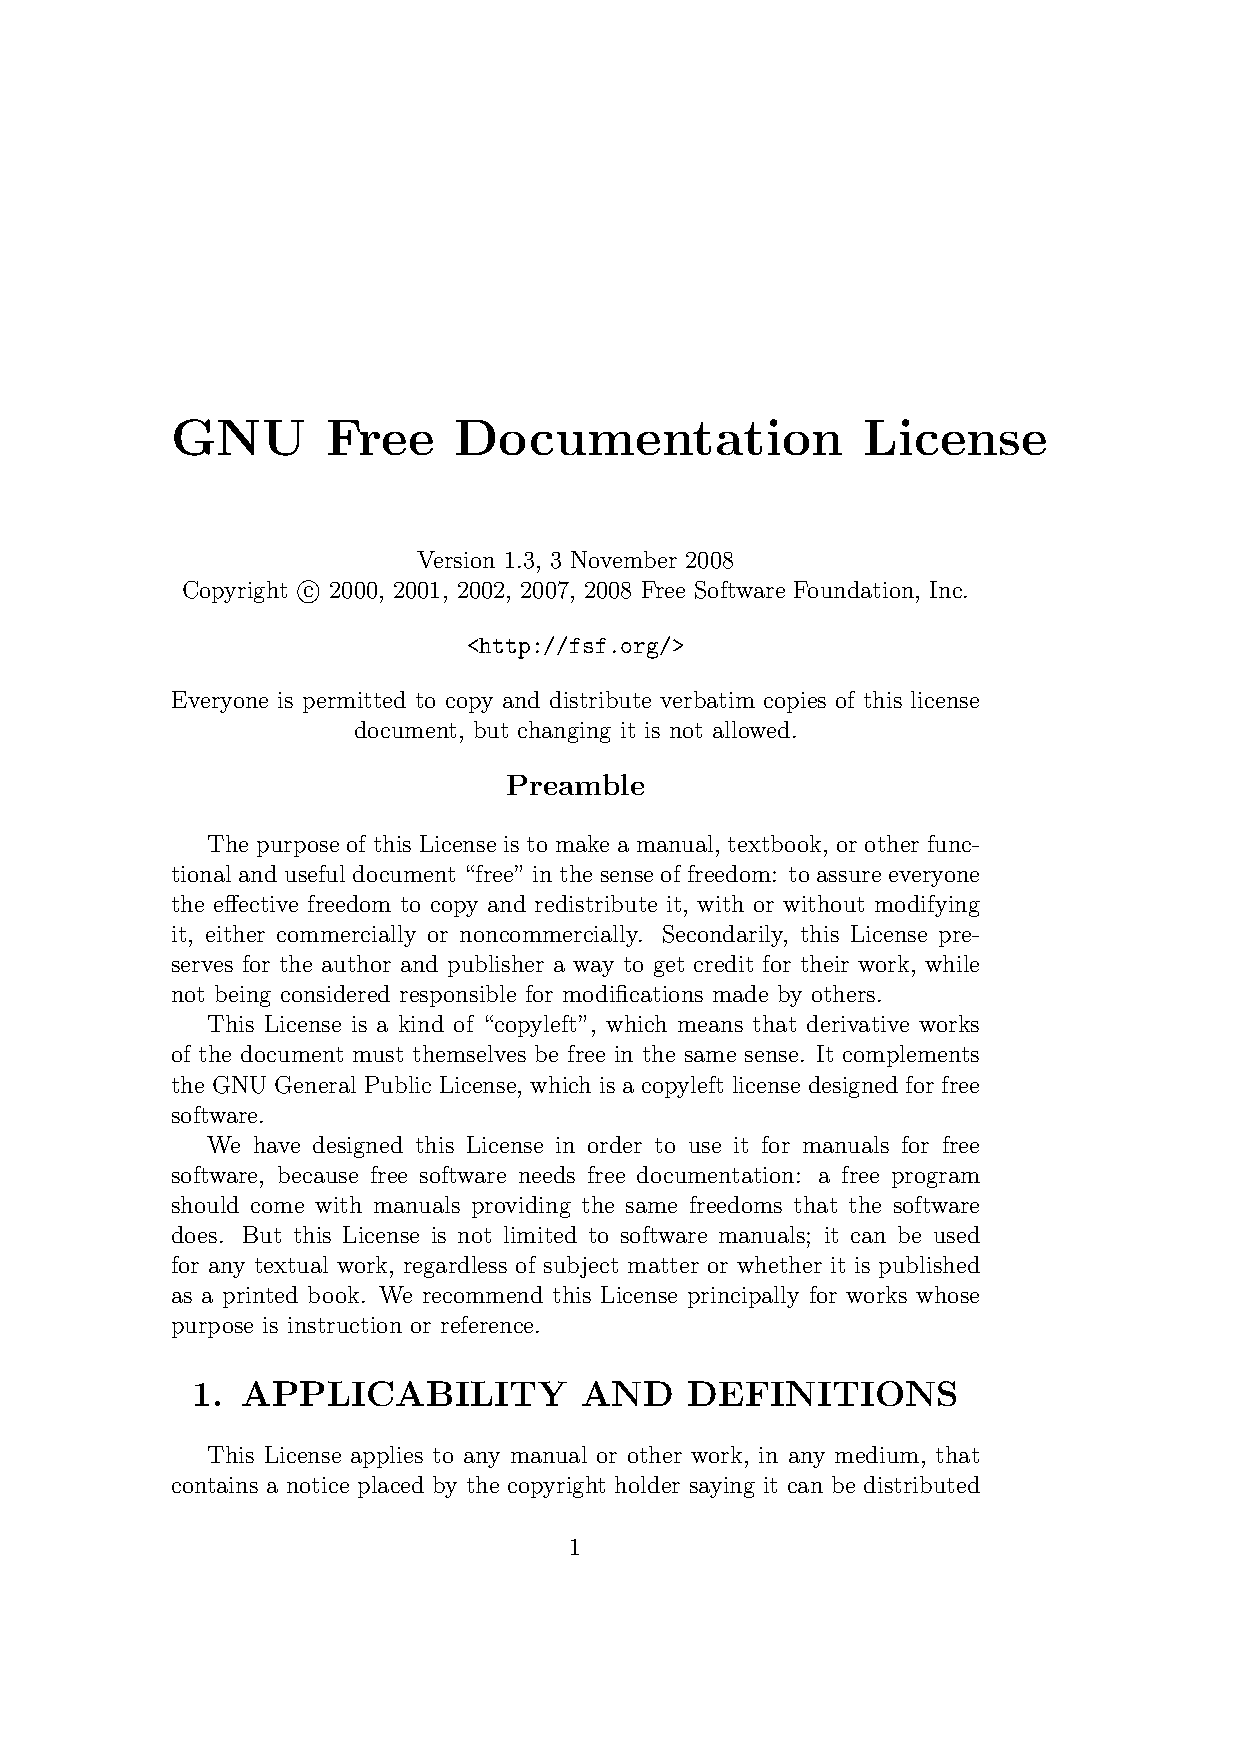
\includepdf[pages=-]{fdl.pdf}
\newpage
\begin{center}
\textbf{\Large EnDaBi Licenses}
\end{center}
\begin{center}
Our Documentation is (as explained above) licensed under the GNU Free Documentation License.
\end{center}
\begin{center}
However, our source Code is Licensed under Different Licenses.
\end{center}
\newpage
 \begin{center} \textbf{\Large Legal} \end{center}
  \begin{center}
  \begin{normalsize}
  This Document is a Manual for a collection of Software Source Code, which along with the Documentation, was put together by a small team of young Engineers as a third year project at  
  \end{normalsize}
  \end{center} 
  \begin{center}
  Tishreen University, Latakia, Syria.
  
  \end{center} 
 
 \begin{center}
   \begin{normalsize}
  The Code Implements well known \textbf{Generic} Mathematical and Computational algorithms, using \textbf{Free Open Sourced} Programming Languages. Compiled and tested on \textbf{Free Open Sourced} Platforms using \textbf{Free Open Sourced} Software.
    \end{normalsize}
     \end{center} 
     \begin{center}
        \begin{normalsize}
  Our Work does \textbf{NOT} Include any Close-Source or Propriety Software.
  \end{normalsize}
     \end{center} 
     \begin{center}
             \begin{normalsize}
             
  \newpage
  Some of our Combined Implementations are Genuine as in Different. However, the Idea Behind the Project and the Individual Implementations of the mathematical algorithms and formulas are all \textbf{Generic}. Which means there might be huge similarities with some of the works out there in the world.
    \end{normalsize}
     \end{center} 
     \begin{center}
    \begin{normalsize}

  In case that happens, if the resemblance is uncanny, we are willing to re-implement.
  In the case that happens, please contact aly.shmahell@gmail.com and there will be a dialogue once we're able to read the email and respond.
  \end{normalsize}
     \end{center} 
     \begin{center}
         \begin{normalsize}
  \textbf{Please Notice} This does not mean we're open to \textbf{trolling}. any attempt to troll our work or drag us into an unlawful debate of ownership will \textbf{NOT be tolerated}.
  
  \end{normalsize}
   \end{center} 

\newpage
\begin{center}
\textbf{\Large Disclaimer}
\end{center}
\begin{center}
THE SOFTWARE IS PROVIDED "AS IS", WITHOUT WARRANTY OF ANY KIND,
EXPRESS OR IMPLIED, INCLUDING BUT NOT LIMITED TO THE WARRANTIES OF
MERCHANTABILITY, FITNESS FOR A PARTICULAR PURPOSE AND NONINFRINGEMENT.
IN NO EVENT SHALL THE AUTHORS OR COPYRIGHT HOLDERS BE LIABLE FOR ANY
CLAIM, DAMAGES OR OTHER LIABILITY, WHETHER IN AN ACTION OF CONTRACT,
TORT OR OTHERWISE, ARISING FROM, OUT OF OR IN CONNECTION WITH THE
SOFTWARE OR THE USE OR OTHER DEALINGS IN THE SOFTWARE.
\end{center}
\begin{center}
\textbf{\large USE AT YOUR OWN RISK.}
\end{center}
\newpage
\begin{center}
The Intent of this Project is to serve man kind, tackling problems with privacy and lawful access.
It's is expected to be used in that manner.
\end{center}
\begin{center}
We are \textbf{NOT} liable or responsible for any misuse of our Project.
\end{center}


\newpage
\begin{center} \textbf{\Large About The Authors} \end{center}
\begin{center}
We are Syrian nationals, who consider themselves citizens of their Country and the World.
\end{center}
\begin{center}
\begin{small}
Below is the list of authors and their contact  info :
\end{small}
\end{center}
\begin{center}
\begin{scriptsize}
 \begin{tabular}{|c | c|} 
 \hline
 Name & Contact \\ [0.5ex] 
 \hline\hline
 Aly Shmahell & aly.shmahell@gmail.com \\ 
 \hline
 Ruaa Sleiman  & ruaa.s.sleiman@gmail.com \\
 \hline
 Elias Soud & Thegamebest21es@gmail.com \\
 \hline
 Wassim Ali & wali91350@gmail.com \\
 \hline
 Motea Rahmoon &  Mrahmoon1994@gmail.com \\ [1ex] 
 \hline
 Alya Salman & el57la.9595@gmail.com\\
 \hline
\end{tabular}
\end{scriptsize}
\end{center}
\newpage
\begin{center}
\textbf{\Large Special Thanks}
\end{center}
\begin{center}
We give our thanks to those who have helped us :
\end{center}
\begin{center}
\textbf{Eng. Sami Abobala} from Tishreen University whose patience and assistance were crucial to our success.
\end{center}
\begin{center}
\textbf{Professor. Dr.Ing. Christof Paar} from Ruhr-Universität Bochum, whose work we've built upon. and for his kindness in allowing us to use parts of his slides in our documentation.
\end{center}
\newpage
\begin{center}
\textbf{\Large Introduction}
\end{center}
\begin{center}
The caveman, the life choice he made to settle down from hunting and gathering provided him with more security inside his cave. but it limited his freedom to roam vast lands.
\end{center}
\begin{center}
The same aspect can be found in modern society.
If a company decreases its security measures on its entrances, the employees can get in and out faster (not having to pull so many cards out, remember so many passwords and such), but it loses some of its security points. and vice versa.
\end{center}
\begin{center}
\textbf{The EnDaBi Project} tackles that problem, and tries to find balance between security and mobility.
\end{center}
\begin{center}
By utilizing state of the art schemes in Encryption, Database and Biometrics technologies and embedding them all into one efficient and coherent library or suite. 
\end{center}
\begin{titlepage}
\begin{center}
\textbf{\Large About The Project}\end{center}
\begin{center}
The premise of the project is simple.
For starters, we're focusing on Encryption.
We spent a fair amount of time searching for material that serve that particular purpose.
\end{center}
\begin{center} We found those published by Professor Christof Paar to be most suitable for implementing and most easy to understand.
\end{center}
\newpage
\begin{center}
\textbf{\Large The Current Project Steps :}
\end{center}
\begin{center}
1) Choosing the RSA algorithm for implementation. for the sake of mobility and security (it being an Asymmetric Cryptographic Scheme).
\end{center}
\begin{center}
2) Trying to make the Implementation as Simple and Usable as possible.
\end{center}
\begin{center}
3) Trying to Enhance Speed and Efficiency.
\end{center}
\begin{center}
4) Porting the Library to as many languages and platforms as possible.
\end{center}
\end{titlepage}
\newpage
\begin{center}
\textbf{\Large Cryptography}
\end{center}
\begin{center}
Cryptography is a science that deals with Rendering Information that is available for everyone to see,and make it such that only a few can understand.
\end{center}
\begin{center}
Cryptography can be divided into a handful of Classifications.
\end{center}
\includepdf[pages=6]{paar1.pdf}
\newpage
\begin{center}
\textbf{\Large Symmetric Cryptography}
\end{center}
\begin{center}
Symmetric Cryptography is a classification in which a \textbf{Shared Key} is exchanged prior to Encryption.
\end{center}
\begin{center}
The \textbf{Key} is used for both \textbf{Encryption and Decryption}.
\end{center}
\begin{center}
The \textbf{Key} must be Exchanged over a \textbf{secure channel} or else if captured it will be used by a \textbf{Malicious Third Party} to decrypt the Encrypted message.
\end{center}
\newpage
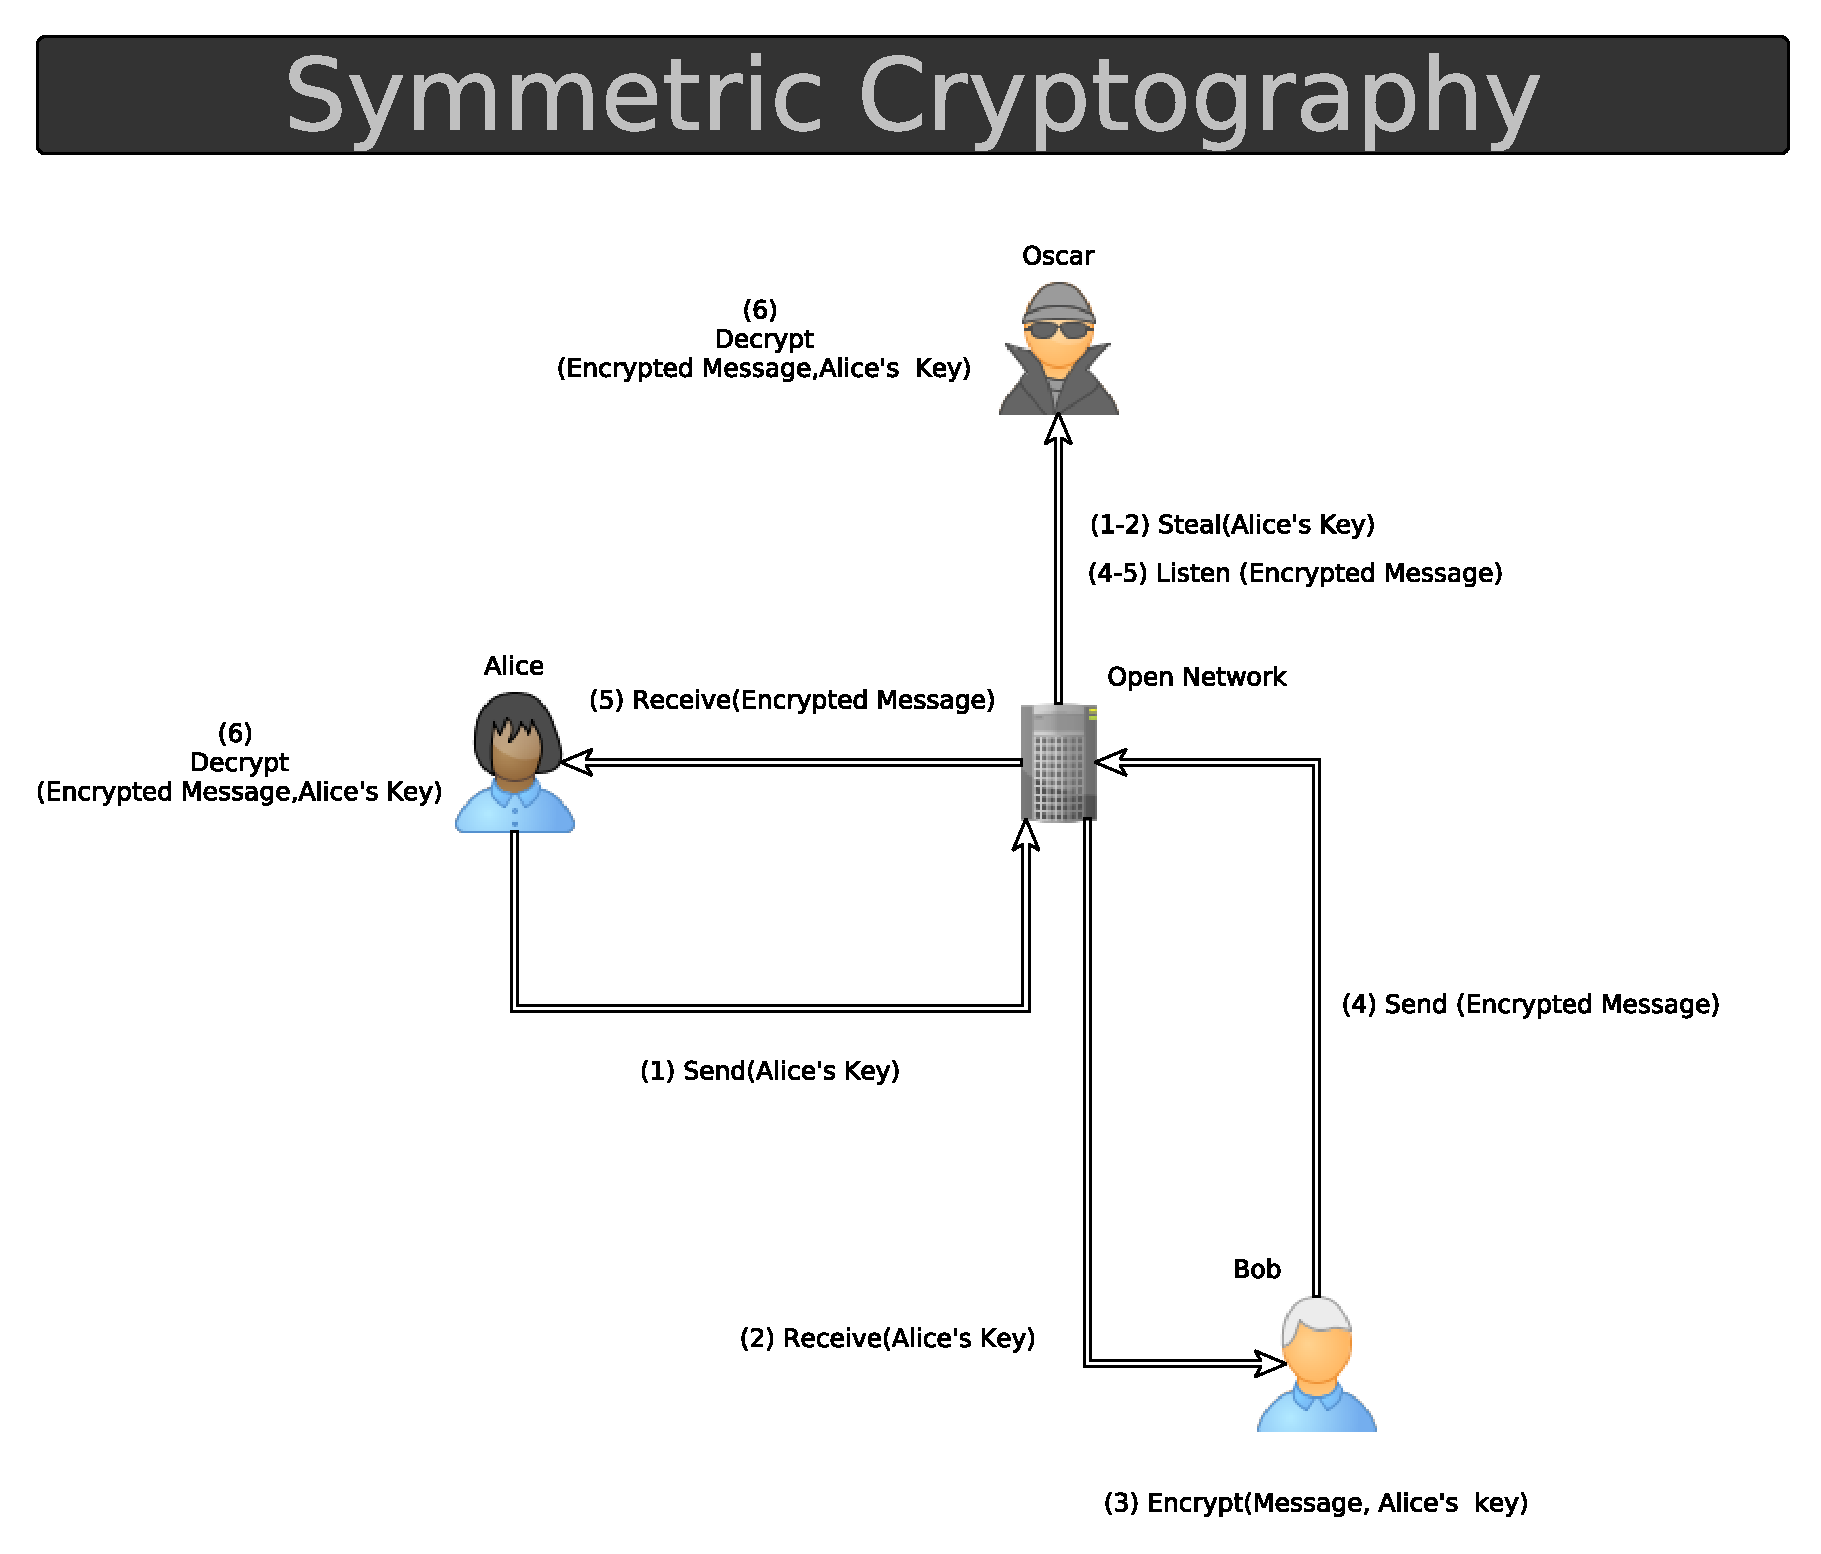
\includepdf{Symmetric-Cryptography.pdf}
\newpage
\begin{center}
\textbf{\Large Asymmetric Cryptography}
\end{center}
\begin{center}
This Encryption Classification Includes a \textbf{Pair of Keys (Public and Private)}.
\end{center}
\begin{center}
\textbf{The Public Key} is used for \textbf{Encryption} solely.
\end{center}
\begin{center}
\textbf{The Private Key} is used for \textbf{Decryption} solely.
\end{center}
\begin{center}
Only the \textbf{Public Key is Exchanged}.
\end{center}
\begin{center}
If a Malicious Third Party Captures the Public Key, it is of no use to them \textbf{(it can't Decrypt)}.
\end{center}
\newpage
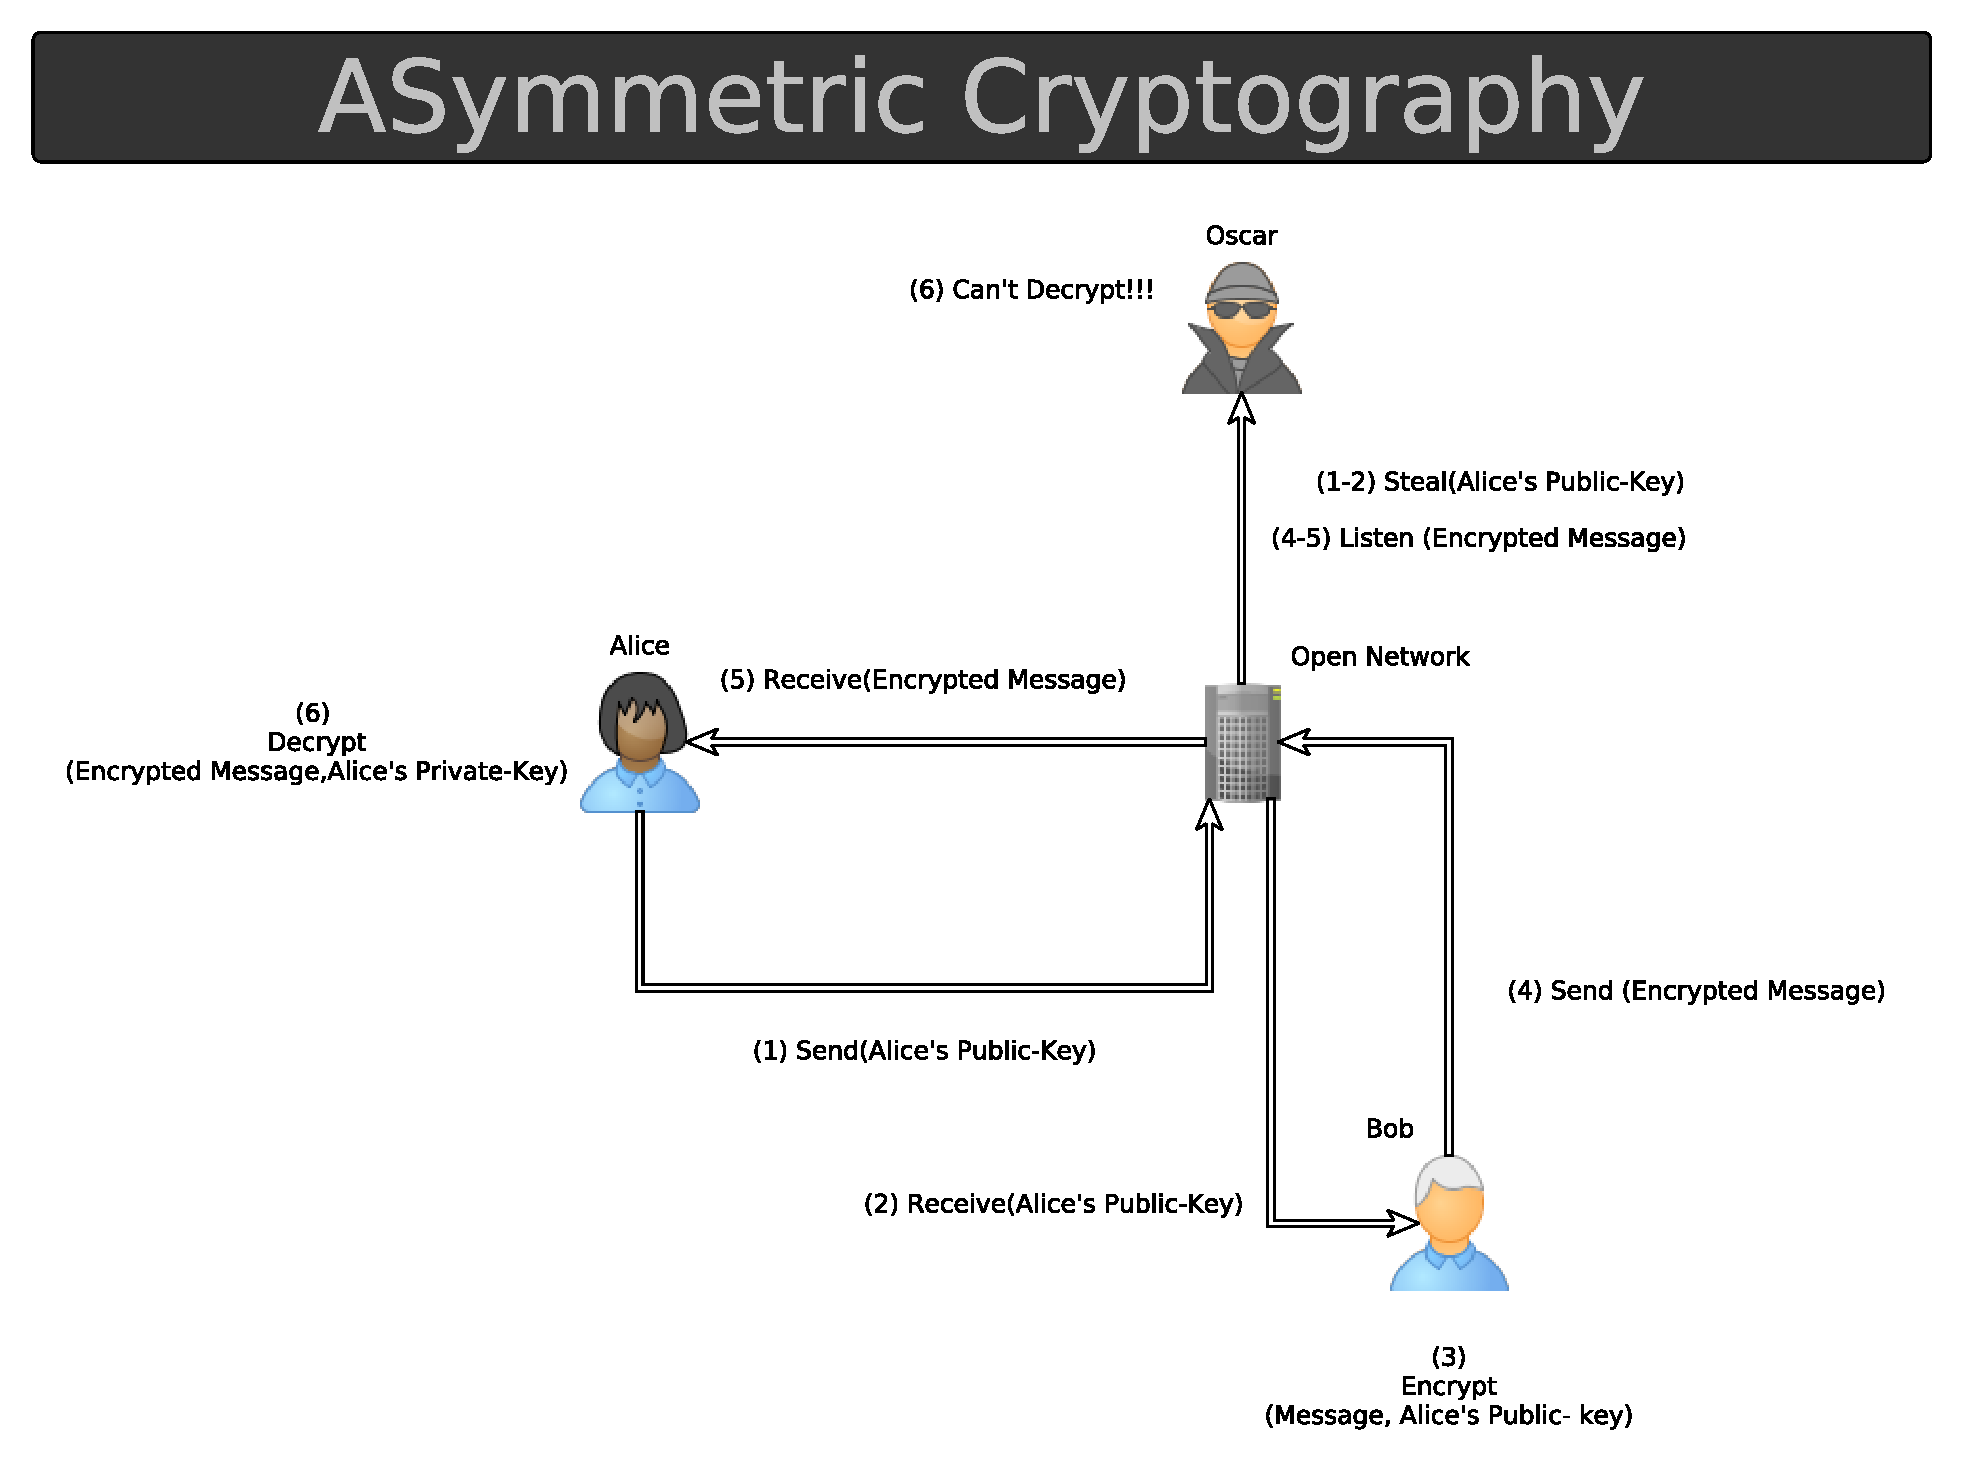
\includepdf{Asymmetric-Cryptography.pdf}
\newpage
\begin{center}
\textbf{\Large Mathematical Background}
\end{center}
\begin{center}
The RSA Algorithm utilizes a number of Well known mathematical Methods and Formulae to achieve a Successful and Secure Encryption/Decryption.
\end{center}
\begin{center}
Those are :
\end{center}
\begin{center}
1) The Euclidean Algorithm.
\end{center}
\begin{center}
2) The Extended Euclidean Algorithm.
\end{center}
\begin{center}
3) Euler's Phi Function.
\end{center}
\begin{center}
4) Fermat's Little Theorem.
\end{center}
\begin{center}
5) Euler's Theorem.
\end{center}
\begin{center}
6) Binary Exponentiation (Square-and-Multiply).
\end{center}
\begin{center}
7) Primality Testing.
\end{center}
\newpage
\begin{center}
\textbf{\Large The Eucledian Agorithm}
\end{center}
\begin{center}
This Algorithm Computes the Greatest Common Divisor of $ r_{0} $ and $ r_{1} $. $ gcd(r_{0},r_{1}) $.
\end{center}
\begin{center}
It does so by following these simple steps :
\end{center}
\begin{center}
1) Test if $ (r_{1} == 0) $, if that's the case, then the final answer is the current $ r_{0} $.
\end{center}
\begin{center}
2) Make $ Temp = r_{1} $
\end{center}
\begin{center}
3) Make $r_{1} = r_{0} \bmod r_{1}$
\end{center}
\begin{center}
4) Make $ r_{0} = Temp $
\end{center}
\begin{center}
5) Repeat Recursively.
\end{center}
\newpage
\begin{center}
\textbf{\Large The Extended Eucledian Algorithm}
\end{center}
\begin{center}
Suppose $ gcd(r_{0},r_{1}) = 1 $ .
\end{center}
\begin{center}
The theory states that you can write that as the following : 
\end{center}
\begin{center}
$ gcd(r0,r1) = s*r_{0} + t*r_{1} $
\end{center}
\begin{center}
Just like the Euclidean Algorithm, we go on calculating the $ gcd $ recursively,making 
\end{center}
\begin{center}
$r_{i}  = r_{i-2} \bmod r_{i-1}$
\end{center}
\begin{center}
$q_{i-1} = (r_{i-2} - r_{i} )/r_{i-1}$
\end{center}
\begin{center}
$ t_{i} = t_{i-2}-q_{i-1}*t_{i-1} $
\end{center}
\begin{center}
until we reach : 
\end{center}
\begin{center}
 $ gcd(r_{0},r_{1}) \equiv 1 $
\end{center}
\begin{center}
at that point $ t=t_{i-1} $
\end{center}
\begin{center}
now we submit the equation to the modulo operation :
\end{center}
\begin{center}
$ gcd(r_{0},r_{1}) \equiv 1 \equiv s*r_{0} + t*r_{1} $
\end{center}
\begin{center}
$ 1 \bmod r_{0} \equiv (s*r_{0} + t*r_{1}) \bmod r0 $
\end{center}
\begin{center}
$ 1 \bmod r_{0} \equiv t*r_{1} \bmod r_{0} $
\end{center}
\begin{center}
and since : $ 1 \bmod r_{0} \equiv r_{1}^{-1}*r_{1} \bmod r0 $
\end{center}
\begin{center}
then : $ r_{1}^{-1} \equiv t $
\end{center}
\begin{center}
And That is \textbf{One} way to calculate the \textbf{Modular Inverse}
\end{center}
\newpage
\includepdf[pages=25-28] {paar2.pdf}
\includepdf[pages=11-12] {paar3.pdf}
\newpage
\begin{center}
\textbf{\Large Primality Testing}
\end{center}
\begin{center}
There are many ways to determine whether integer P is prime or not.
\end{center}
\begin{center}
One way is we make sure P is prime, By factorization.
\end{center}
\begin{center}
The other is depending on \textbf{Equivalence Rules} that only apply to primes. and Testing whether these Rules apply to P or not.
\end{center}
\begin{center}
If They do, then P is \textbf{probably} Prime.
\end{center}
\begin{center}
If They don't, then P is \textbf{definitely} Composite.
\end{center}
\newpage
\begin{center}
\textbf{\Large Using Sieves for Factorization}
\end{center}
\begin{center}
Sieves are a great way to Shrink the amount of time needed to test the primality of \textbf{Many or More} test cases.
\end{center}
\begin{center}
A Sieve is a Boolean Array, that uses the Index to signal the number we're storing, and uses the boolean value to signal Primality (1 being Prime, 0 being Composite)
\end{center}
\begin{center}
The Array is initialized with 1. as in all numbers are initially considered Primes.
\end{center}

\begin{center}
Then we start going through numbers (indexes).
\end{center}
\begin{center}
 for each index that has a value of 1, do the following:
\end{center}
\begin{center}
go through all the indexes that are multiples of that prime index, and switch their values to 0.
\end{center}
\newpage
\begin{center}
\textbf{\Large Sieve Tricks}
\end{center}
\begin{center}
Consider the Following :
\end{center}
\begin{center}
1) For a given Prime index, all multiples of that index up until $ index^2 $ are switched to composites (value to 0), by the \textbf{Previous Prime} index \textbf{Passes}.
\end{center}
\begin{center}
Therefor : only switch the multiples of a Prime index that are above $ index^2 $ .
\end{center}
\begin{center}
2) All Prime indexes needed to determine the primality of an index are below $ \sqrt[2]{index} $.
\end{center}
\begin{center}
Therefor : keep going through prime indexes until index = $\sqrt[2]{Array_{limit}}$ .
\end{center}
\newpage
\begin{center}
\textbf{\Large Prime Rules}
\end{center}
\begin{center}
Consider a Prime number P, it can be written as :
$ P = (r_{1} * r_{2} *....* r_{i})+1$
\end{center}
\begin{center}
where : $r_{1}.......r_{i} $ is a factor of $ P-1 $ .
\end{center}
\begin{center}
Take a random number a where :
\end{center}
\begin{center}
$ a>1 $ and $ a<P  \Rightarrow  \gcd(P,a)=1 $ .
\end{center}
\begin{center}
now find the result of this equation :
\end{center}
\begin{center}
$ a^{P-1}=?\bmod P $ .
\end{center}
\begin{center}
$ a^{(r_{1} * r_{2} *....* r_{i})}= ?\bmod P $ .
\end{center}
\begin{center}
$ ((a^{r_{1}})^{r_{2}})^{r_{i}} = ?\bmod P $
\end{center}
\begin{center}
with $ answer = (a^{r_{i}} \bmod P) \in [1...P-1] $
\end{center}
\begin{center}
We've got P-1 tries, and each try produces a different $ answer $ (since the modulus operation is cyclic and $ \gcd(P,a)=1 $) until we reach $ a^{r_{i}} = 1 \bmod P $
\end{center}
\begin{center}
at that point $ 1^{r_{i}} \equiv 1 \bmod P $
\end{center}
\begin{center}
The above proves \textbf{Fermat's Little Theorem}.
\end{center}
\begin{center}
It makes it that if a given number P passes the above Equivalence Rule, then it's a \textbf{Probable Prime}.
\end{center}
\begin{center}
But also if we consider $ a^{P} $, by a few steps of mathematical manipulation we derive that :
\end{center}
\begin{center}
$ a^{P} \equiv a \bmod P $
\end{center}
\begin{center}
if we multiply both sides by $ a^{-1} $ : $ a^{P}*a^{-1} \equiv a*a^{-1} \bmod P $
\end{center}
\begin{center}
$ 1 \equiv a*a^{-1} \bmod P \Rightarrow a^{P-1} \equiv a^{-1}$ 
\end{center}
\begin{center}
and that is a \textbf{Second} way to calculate the
\end{center}
\begin{center}
\textbf{Modular Inverse} .
\end{center}
\newpage
\includepdf[pages=5-7]{paar3.pdf}
\newpage
\begin{center}
\textbf{Why the RSA is Secure!}
\end{center}
\begin{center}
1) To calculate the private Key Efficiently you need to use the Extended Euclidean Algorithm on the e and $ \phi(n) $ .
\end{center}
\begin{center}
2) to Calculate $ \phi(n) $ you  need to have $ p $ and $ q $.
\end{center}
\begin{center}
3) The only way to get $ p $ and $ q $ from a non-secure channel is by getting $ n $ (which is public).
\end{center}
\begin{center}
4) Factoring $ n $ proves Impractical for $ (>1024) $ bit Integers ,by today's standard computing power.
\end{center}
\newpage
\begin{center}
\textbf{\Large RSA's Shortcomings}
\end{center}
\begin{center}
1) When choosing a relatively small Exponent $ e $ as a Public-Key, if $ message^{e} < modulus $, then by deduction :

 $message^{e} \equiv message^{e} \bmod modulus $.

And the message can be regenerated using $ message = \sqrt[e]{message^{e}} $ 

Therefor : Avoid Relatively Small numbers when choosing a Public-Key.
\end{center}
\begin{center}
2) Attackers can Encrypt a Predicted Plain text with the Public-Key, and Compare it to the Original Encrypted text.

Solution : \textbf{Padding} the Text Message prior to Encryption with Random Values.
\end{center}
\newpage
\begin{center}
\textbf{\Large EnDaBi Implementations}
\end{center}
\begin{center}
These Implementations include :
\end{center}
\begin{center}
. The EnDaBi RSA Core Library.
\newline . a Console Demo showcasing the Library's main functions.
\newline . a GUI Demo showcasing the Library's main functions.
\newline  . an Example Segmented Sieve Program
\newline . a Small java program that utilizes built-in primality testing.
\newline . a make file used to compile the demos.
\end{center}
\newpage
\begin{center}
\textbf{\Large Toolkits, Libraries and Programming Languages We Used}
\end{center}
\begin{center}
\textbf{C++} : Strongly typed, Fast and efficient, library extended Programming-Language.
\end{center}
\begin{center}
\textbf{D} : Strongly typed, Fast and efficient Programming-Language with Syntax Similar to that of C and Java.
\end{center}
\begin{center}
\textbf{Java} : Strongly typed, byte-code compiled programming language that devotes to binary portability (compile once, run everywhere).
\end{center}
\begin{center}
\textbf{FLTK} : Fast Light Tool Kit ("FLTK", pronounced "fulltick") is a C++ graphical user interface toolkit for the X Window System, MacOS, and Microsoft  Windows that supports OpenGL.
\end{center}
\begin{center}
\textup{ENDABI RSA DEMO GUI} is based in  part  on  the  work  of  the  FLTK project \url{http://www.fltk.org}.
\end{center}
\newpage
\begin{center}
\textbf{LaTeX} : is a high-quality typesetting system; it includes features designed for the production of technical and scientific documentation. LaTeX is the de-facto standard for the communication and publication of scientific documents. 
\end{center}
\begin{center}
\textbf{InfInt} : Arbitrary-Precision Integer Arithmetic Library. licenced under LGPL 2.1. Copyright (C) 2013 Sercan Tutar
\end{center}
\begin{center}
\url{code.google.com/p/infint/}
\end{center}
\newpage
\begin{center}
\textbf{\Large Software we Used}
\end{center}
\begin{center}
\textbf{Ubuntu 14.04 LTS} : Free and Open Source Linux-Based Operating System.
\end{center}
\begin{center}
\textbf{GCC} : GNU project C and C++ compiler.
\end{center}
\begin{center}
 \textbf{GDC} : A GCC-based compiler for the D language.
\end{center}
\begin{center}
\textbf{Javac} : Java programming language compiler.
\end{center}
\begin{center}
\textbf{TeXstudio} : is a LaTeX editor with a graphical user  interface.
\end{center}
\begin{center}
\textbf{Code::Blocks} : The open-source, cross-platform IDE.
\end{center}
\begin{center}
\textbf{SciTE} : a programmers text editor
\end{center}
\begin{center}
\textbf{Vim} : is a text editor that is upwards compatible to Vi.  It can be used to edit all kinds of plain text.  It is especially useful  for editing programs.
\end{center}
\newpage
\begin{center}
\textbf{Eclipse} : extensible tool platform and Java IDE.
\end{center}
\begin{center}
\textbf{ nano} : is  a small, free and friendly editor which aims to replace Pico, the default editor included in the non-free Pine package.
\end{center}
\begin{center}
\textbf{make} : GNU make utility to maintain groups of programs
\end{center}
\begin{center}
\textbf{Git} : is a fast, scalable, distributed revision control system with an unusually rich command set that provides both high-level operations and full access to internals.
\end{center}
\begin{center}
\textbf{yEd} : is a powerful desktop application that can be used to quickly and effectively generate high-quality diagrams.
\end{center}
\newpage
\begin{center}
\textbf{\Large How To Use Our Software}
\end{center}
\begin{center}
1) This Installation process was tested on Ubuntu 14.04 LTS.
\end{center}
\begin{center}
2) \textbf{Install Prerequisites}
\begin{center}
In Terminal, Type :
\end{center}
\begin{BVerbatim}
sudo apt-get install gcc g++ gdc openjdk-7-jdk
   vim libfltk1.3-dev fltk1.3 fltk1.3-doc
         build-essential make git 
\end{BVerbatim}
\end{center}
\begin{center}
3) \textbf{Pull EnDaBi Sources from Github}
\begin{center}
In Terminal, Type :
\end{center}
\begin{BVerbatim}
git clone https://github.com/EnDaBi/EnDaBi.git
\end{BVerbatim}
\end{center}
\newpage
\begin{center}
4) \textbf{Navigate to the EnDaBi Folder}
\begin{center}
In Terminal, Type :
\end{center}
\begin{BVerbatim}
cd EnDaBi
\end{BVerbatim}
\end{center}
\begin{center}
5) \textbf{Compile the Sources}
\begin{center}
In Terminal, Type :
\end{center}
\begin{BVerbatim}
make
\end{BVerbatim}
\end{center}
\begin{center}
6) \textbf{Run Demos}
\end{center}
\begin{center}
In Terminal, Type :
\end{center}
\begin{center}
\centering
\begin{BVerbatim}
./ENDABI_RSA_DEMO_GUI
          
          or
          
  ./ENDABI_RSA_DEMO
\end{BVerbatim}
\end{center}
\newpage
\begin{center}
\textbf{\Large What's Next}
\end{center}
\begin{center}
\textbf{Regarding the RSA Core :}
\end{center}
\begin{center}
1) Implementing the Chinese Remainder Theorem for Faster Private Key Exponentiation (Decryption).

2) Implementing Our Own BigInteger Library.

3) Implementing our Own Padding System.

4) Implementing Our own Primality Testing Classes.
\end{center}
\begin{center}
\textbf{Regarding the Project :}

1) Adding more Encryption Schemes.

2) Developing Database Classes.

3) Developing Biometrics Classes.
\end{center}
\newpage
\begin{center}
\textbf{\Large References}
\end{center}
\begin{center}
\begin{BVerbatim}
[1]        Paar, C., and Pelzl, J.
         Understanding Cryptography
  A Textbook for Students and Practitioners.
                  2010.
         www.crypto-textbook.com
        Prof. Dr.-Ing. Christof Paar 
        Chair for Embedded Security
          Ruhr-Universitat Bochum
             D - 44780 Bochum.
\end{BVerbatim}
\end{center}
\end{document}